\documentclass{jarticle}
\usepackage[dvipdfmx]{graphicx}
\topmargin       -10.0mm
\oddsidemargin   -0.4mm
\evensidemargin  -0.4mm
\headheight       0.0mm
\headsep          0.0mm
\footskip        10.0mm
%
\textheight     260.0mm
\textwidth      170.0mm
%
\setlength{\parindent}{1zw}
%
\usepackage{graphicx}
\usepackage{multirow}
\usepackage{wrapfig}
\makeatletter
\def \fgcaption{\def \@captype{figure} \caption}
\def \tbcaption{\def \@captype{table} \caption}
\makeatother
\def \figurename{Fig.}
\def \tablename{Table}
%
\def\topfraction{.99}
\def\bottomfraction{.99}
\def\textfraction{.01}
\def\floatpagefraction{.99}
%
\pagestyle{empty}
%
\begin{document}
%
\begin{center}
 \begin{tabular}{|c|c|c|} \hline
  \parbox{50mm}{\vspace{1mm} \centering{\Large\bf 2026/06/18}} & 
  \parbox{55mm}{\vspace{1mm} \centering{\Large\bf B4　堀田裕樹}} & 
  \parbox{50mm}{\vspace{1mm} \centering{\Large\bf No.~10}}
  \\ [2mm] \hline
%
  \multicolumn{3}{|c|}{%
   \parbox{155mm}{\centering\Large\bf
    \vspace{1mm}
    シミュレーションパラメータの拡充と実験データによる妥当性検証
   }
  }
  \\ [2mm] \hline\hline
%
  \multicolumn{3}{|c|}{%
   \parbox{155mm}{\large\vspace{1mm}
%
    {\Large\bf 今月の目標}
%
    \begin{itemize}
     \item シミュレーションの解析
    \end{itemize}
%
    {\Large\bf 進捗の要点}
%
    \begin{itemize}
     \item 傷の深さ（depth）のシミュレーション範囲を $0.20$ mm まで拡大
     \item ピーク同期（Time-align）による波形およびスペクトルの妥当性検証
    \end{itemize}
%
    {\Large\bf 今後の実施事項}
%

%
   }
  }
  \\ [2mm] \hline
 \end{tabular}
%
\end{center}
%

\begin{center}
  \begin{minipage}[b]{0.49\linewidth}
    \centering
    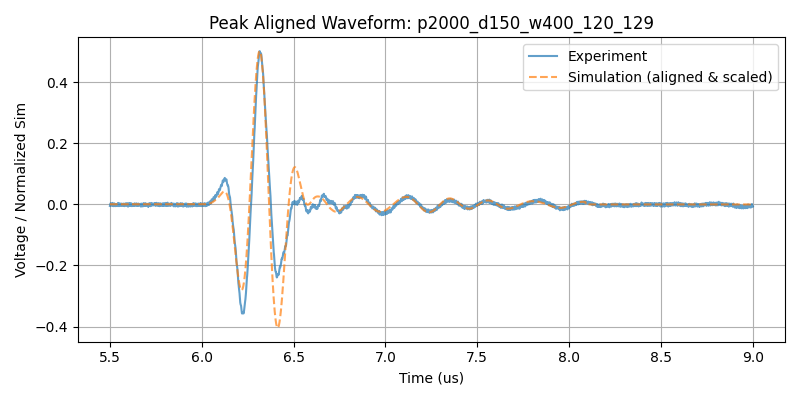
\includegraphics[width=6.8cm]{../../vscode/simulation/data/comparison_plots/compare_wave_p2000_d150_w400_120_129.png}
    \vspace{-2mm}
    \fgcaption{Waveform Comparison (p2000\_d150\_w400)}
  \end{minipage}
  \begin{minipage}[b]{0.49\linewidth}
    \centering
    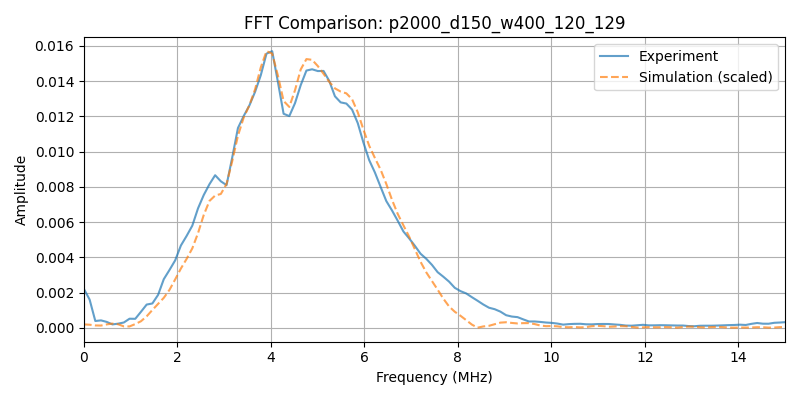
\includegraphics[width=6.8cm]{../../vscode/simulation/data/comparison_plots/compare_fft_p2000_d150_w400_120_129.png}
    \vspace{-2mm}
    \fgcaption{FFT Comparison (p2000\_d150\_w400)}
  \end{minipage}
\end{center}

\begin{center}
  \begin{minipage}[b]{0.49\linewidth}
    \centering
    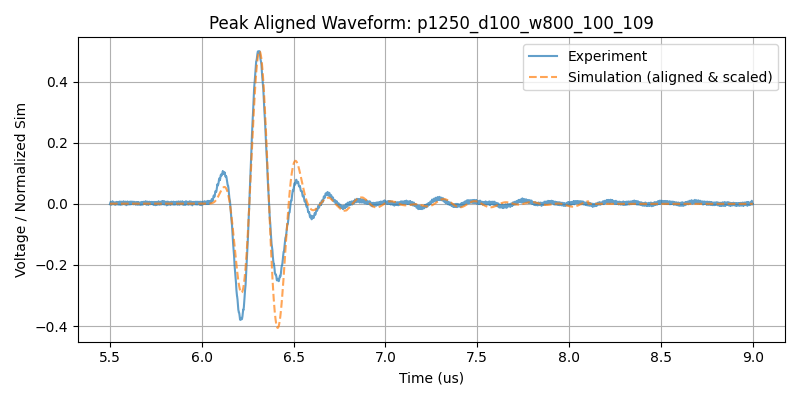
\includegraphics[width=6.8cm]{../../vscode/simulation/data/comparison_plots/compare_wave_p1250_d100_w800_100_109.png}
    \vspace{-2mm}
    \fgcaption{Waveform Comparison (p1250\_d100\_w800)}
  \end{minipage}
  \begin{minipage}[b]{0.49\linewidth}
    \centering
    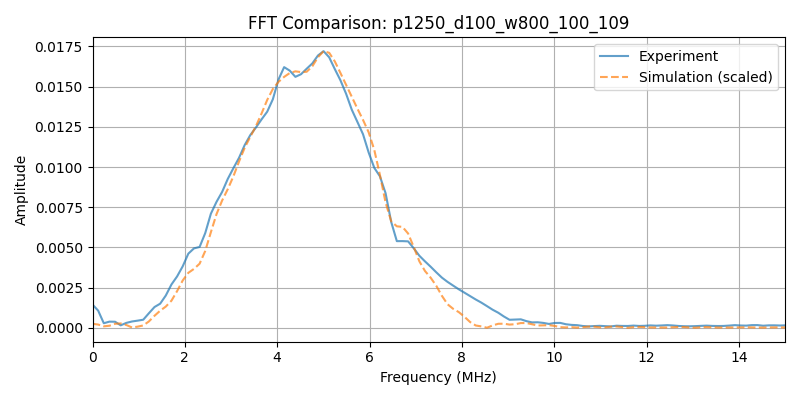
\includegraphics[width=6.8cm]{../../vscode/simulation/data/comparison_plots/compare_fft_p1250_d100_w800_100_109.png}
    \vspace{-2mm}
    \fgcaption{FFT Comparison (p1250\_d100\_w800)}
  \end{minipage}
\end{center}

%
\end{document}
